\subsubsection{UserInterface} \label{sec:c1}
Componente che si occupa di rappresentare il livello \textit{user interface} nell'architettura three tier dell'applicazione. Esso contiene l'interfaccia grafica visibile all'utente, ed è responsabile della presentazione dei dati e della corretta interpretazione degli eventi utente e del loro inoltro nei livelli inferiori. Contiene le finestre del programma, cioè finestra principale, finestra di configurazione, finestra di calibrazione. \\
\begin{figure}[!h] 

        \centering 

        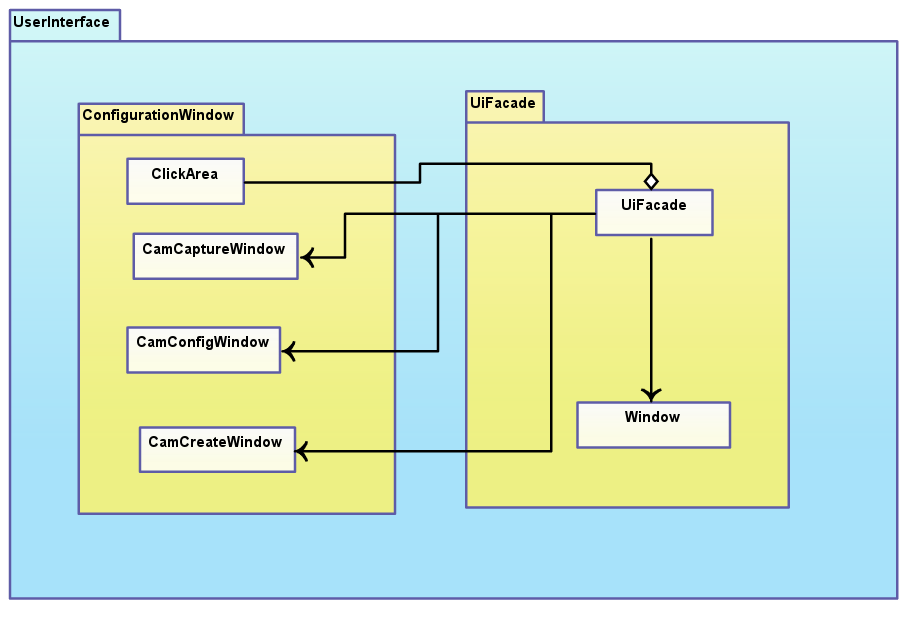
\includegraphics[scale=0.4]{./images/c1.png} 

        \caption{C1 - UserInterface} 

        \label{fig:c1}

        \end{figure} 

Relazioni con altri componenti: 
\begin{description} 
\item [\textbf{BusinessLayer}]
Il livello di presentazione (UI) utilizza il livello logico per inoltrare e quindi rispondere agli eventi utente. Ogni richiesta infatti viene delegata al livello sottostante il quale è responsabile per la risoluzione e la risposta ad essa 
\end{description} 

\subsubsection{UserInterface::ConfigurationWindow} \label{sec:c1.1}
Tale componente si occupa della presentazione delle finestre di configurazione del sistema. \\
Classi contenute nel componente: 
\begin{itemize} 
\item \textbf{ClickArea}
\begin{description}
\item [\textit{descrizione e utilizzo:}] Rappresenta una finestra dove le coordinate dei click dell'utente vengono memorizzate in dei campi per una successiva elaborazione. Viene utilizzata per il calcolo della matrice omografica che permette la mappatura dei dati di tracking, memorizza le coordinate (relative alla finestra) dei punti cliccati dall'utente affinché possano in seguito essere recuperati ed elaborati
\item [\textit{classi ereditate:}] QLabel
\end{description}
\item \textbf{CamCaptureWindow}
\begin{description}
\item [\textit{descrizione e utilizzo:}] Rappresenta la finestra che aiuta l'utente a salvare (direttamente dallo stream della telecamera) o inserire (dal file system) un frame della telecamera. Viene utilizzata per svolgere tale funzione, offre sia la possibilità di catturare un'immagine dal video stream sia quella di selezionare un file dal disco da utilizzare per il calcolo della \textit{homography matrix}
\item [\textit{classi ereditate:}] QWidget
\end{description}
\item \textbf{CamCreateWindow}
\begin{description}
\item [\textit{descrizione e utilizzo:}] Rappresenta la finestra per l'inserimento di una nuova telecamera. Essa viene utilizzata per l'inserimento di una nuova configurazione relativa ad una telecamera nel sistema. Fornisce all'utente il campo dove inserire il nome della telecamera e segnala l'azione di inserimento 
\item [\textit{classi ereditate:}] QWidget
\end{description}
\item \textbf{CamConfigWindow}
\begin{description}
\item [\textit{descrizione e utilizzo:}] Rappresenta la finestra che permette all'utente di gestire la configurazione delle telecamere. Viene utilizzata per tutte le modifiche di tali informazioni (insert, update, delete) su ogni dato salvato nel database, cioè informazioni di calibrazione, matrice omografica associata, e nome della telecamera
\item [\textit{classi ereditate:}] QWidget
\end{description}
\end{itemize}

\subsubsection{UserInterface::UiFacade} \label{sec:c1.2}
Componente che si occupa della visualizzazione della finestra principale del programma e del corretto inoltro delle richieste e degli eventi provenienti dal livello di \textit{user interface} ai livelli inferiori.\\
Relazioni con altri componenti: 
\begin{description} 
\item [\textbf{ConfigurationWindow}]
Il componente tiene il controllo di tutte le finestre del sistema, quindi utilizza ConfigurationWindow (~\ref{sec:c1.1}) per accedere alle finestre di configurazione. E' responsabile per la loro corretta visualizzazione e l'interpretazione dei loro segnali 
\item [\textbf{Configurer}]
Il componente utilizza le funzionalità messe a disposizione da Configurer (~\ref{sec:c2.1}) per rispondere alle richieste di configurazione dell'utente 
\item [\textbf{Importer}]
Il componente utilizza le funzionalità messe a disposizione da Importer (~\ref{sec:c2.2}) per rispondere alle richieste riguardanti l'importazione dei file .DXF e la loro conversione e visualizzazione. 
\item [\textbf{StatGenerator}]
Il componente utilizza le funzionalità messe a disposizione da StatGenerator (~\ref{sec:c2.3}) per rispondere alle richieste di visualizzazione statistiche o generazione delle stesse 
\item [\textbf{Utility}]
Il componente utilizza le funzionalità messe a disposizione da Utility (~\ref{sec:c2.4}) per svolgere le funzioni di utilità 
\end{description} 

Classi contenute nel componente: 
\begin{itemize} 
\item \textbf{UiFacade}
\begin{description}
\item [\textit{descrizione e utilizzo:}] Rappresenta il facade utilizzato per convogliare in un unico punto tutte le richieste uscenti dal livello di presentazione verso i livelli sottostanti. Essa viene utilizzata per tale scopo, infatti tutte le altre classi di interfaccia segnalano gli eventi utente a UiFacade che si occupa di inoltrare una precisa richiesta ai livelli sottostanti
\item [\textit{classi ereditate:}] QWidget
\end{description}
\item \textbf{Window}
\begin{description}
\item [\textit{descrizione e utilizzo:}] Finestra principale del programma. Contiene i bottoni per l'accesso alle varie funzionalità. Viene caricata all'avvio del sistema e rimane aperta per l'intera durata dell'esecuzione, gestisce gli eventi utente inoltrando i segnali verso i livelli inferiori
\item [\textit{classi ereditate:}] QWidget
\end{description}
\end{itemize}

\subsubsection{BusinessLayer} \label{sec:c2}
Componente che rappresenta il livello \textit{business layer} nell'architettura three tier dell'applicazione. Esso contiene le classi che contengono la logica dell'applicazione, ed è responsabile della corretta risoluzione delle chiamate provenienti dall'\textit{user interface}. Esso è inoltre incaricato di gestire gli errori e di segnalarli.
\\
\begin{figure}[!h] 

        \centering 

        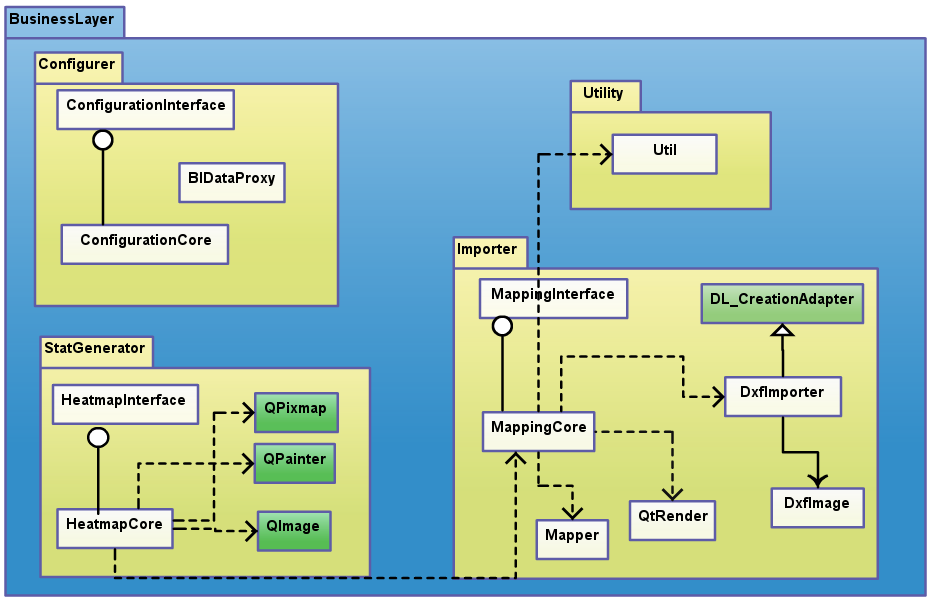
\includegraphics[scale=0.4]{./images/c2.png} 

        \caption{C2 - BusinessLayer} 

        \label{fig:c2}

        \end{figure} 

Relazioni con altri componenti: 
\begin{description} 
\item [\textbf{DataAccessLayer}]
Il livello logico (BL) utilizza il livello di \textit{data access} ogni volta che ha necessità di reperire informazioni memorizzate in un database o di modificarle (select, insert, update, delete). Una volta che ha ottenuto il dato o eseguito l'operazione la interpreta e agisce di conseguenza (stato di errore, corretta terminazione) 
\end{description} 

\subsubsection{BusinessLayer::Configurer} \label{sec:c2.1}
Componente che è responsabile per le funzionalità di configurazione del sistema.\\
Relazioni con altri componenti: 
\begin{description} 
\item [\textbf{DataAccessFacade}]
Utilizza DataAccessFacade (~\ref{sec:c3.1}) per accedere ai dati dell'applicazione. Vi delega le operazioni sul database 
\end{description} 

Classi contenute nel componente: 
\begin{itemize} 
\item \textbf{ConfigurationInterface}
\begin{description}
\item [\textit{descrizione e utilizzo:}] Classe astratta che definisce l'interfaccia per la configurazione delle telecamere del sistema. Viene implementata e i suoi metodi vengono ridefiniti per fornire le funzionalità di configurazione richieste
\end{description}
\item \textbf{ConfigurationCore}
\begin{description}
\item [\textit{descrizione e utilizzo:}] Eredita ConfigurationInterface. Implementa metodi necessari per la configurazione delle telecamere nel sistema. Fornisce i metodi per eseguire inserimento, modifica e cancellazione delle informazioni presenti nelle tabelle del database locale
\item [\textit{classi ereditate:}] ConfigurationInterface
\end{description}
\item \textbf{BlDataProxy}
\begin{description}
\item [\textit{descrizione e utilizzo:}] Fornisce un accesso unificato per il solo recupero (select) dei dati salvati nel sistema. Raggruppa tutti i metodi di selezione necessari al livello di interfaccia per presentare i dati. Viene utilizzata da UiFacade come ponte per l'accesso ai dati presenti nel database
\end{description}
\end{itemize}

\subsubsection{BusinessLayer::Importer} \label{sec:c2.2}
Componente responsabile per le funzionalità di importazione dei file .DXF e la loro conversione e rendering in immagine. \\
Classi contenute nel componente: 
\begin{itemize} 
\item \textbf{MappingInterface}
\begin{description}
\item [\textit{descrizione e utilizzo:}] Classe astratta che definisce l'interfaccia per i metodi di \textit{mapping}. Viene implementata e i suoi metodi vengono ridefiniti per fornire le funzionalità di importazione e generazione della \textit{homography matrix}
\end{description}
\item \textbf{MappingCore}
\begin{description}
\item [\textit{descrizione e utilizzo:}] Ridefinisce MappingInterface. Implementa i metodi necessari per l'importazione e il \textit{mapping} dei dati per renderli direttamente utilizzabili per il calcolo di statistiche. Utilizza i metodi contenuti nelle altre classi del componente (quali \textbf{Mapper}, \textbf{QtRender}, \textbf{DxfImporter})
\item [\textit{classi ereditate:}] MappingInterface
\end{description}
\item \textbf{DxfImage}
\begin{description}
\item [\textit{descrizione e utilizzo:}] Descrive un immagine contenuta in un file di tipo .DXF. Contiene dei riferimenti a delle strutture che rappresentano gli elementi (quelli che vengono importati) contenuti nel file. Viene utilizzata per l'importazione dei file .DXF e per la loro visualizzazione

\end{description}
\item \textbf{DxfImporter}
\begin{description}
\item [\textit{descrizione e utilizzo:}] Eredita la classe astratta fornita dalla libreria dxflib definita per il \textit{parsing} e l'importazione dei file .DXF. Converte le strutture fornite dalla classe nelle strutture proprie del sistema, poi le aggiunge ad un oggetto di tipo DxfImage per la memorizzazione. Viene utilizzata nell'importazione e nel parsing dei file .DXF
\item [\textit{classi ereditate:}] DL_CreationAdapter
\end{description}
\item \textbf{QtRender}
\begin{description}
\item [\textit{descrizione e utilizzo:}] Classe che si occupa di fare il \textit{render} di un'immagine contenuta in una classe di tipo DxfImage su un oggetto di tipo QPixmap (che rappresenta un immagine bitmap sulla quale poter disegnare). Utilizza la classe QPainter per disegnare, e viene utilizzata per la visualizzazione dei file .DXF importati e la loro conversione in formato .PNG
\end{description}
\item \textbf{Mapper}
\begin{description}
\item [\textit{descrizione e utilizzo:}] Classe che raggruppa le funzionalità di \textit{mapping}. Essa viene utilizzata dalle classi che si occupano di della mappatura per l'esecuzione dei metodi basilari che  sono: calcolo della matrice omografica e applicazione della trasformazione ad un punto
\end{description}
\end{itemize}

\subsubsection{BusinessLayer::StatGenerator} \label{sec:c2.3}
Componente responsabile per la generazione delle statistiche di tracking a partire dai dati del sistema. \\
Relazioni con altri componenti: 
\begin{description} 
\item [\textbf{DataAccessFacade}]
Utilizza DataAccessFacade (~\ref{sec:c3.1}) per accedere ai dati dell'applicazione. Recupera le informazioni sui dati per la generazione delle statistiche richieste 
\end{description} 

Classi contenute nel componente: 
\begin{itemize} 
\item \textbf{HeatMapInterface}
\begin{description}
\item [\textit{descrizione e utilizzo:}] Classe astratta che definisce l'interfaccia per le funzionalità di generazione \textit{heatmap}. Viene implementata e i suoi metodi vengono ridefiniti per fornire il metodo di generazione heatmap
\end{description}
\item \textbf{HeatmapCore}
\begin{description}
\item [\textit{descrizione e utilizzo:}] Ridefinisce HeatMapInterface. Implementa i metodi necessari per la generazione dell'\textit{heatmap}. Utilizza un gradiente salvato nella directory di esecuzione del programma per scegliere le gradazioni del colore nella mappa, segnala l'errore se tale file è mancante
\item [\textit{classi ereditate:}] HeatMapInterface
\end{description}
\end{itemize}

\subsubsection{BusinessLayer::Utility} \label{sec:c2.4}
Componente che contiene alcune funzionalità di utility. Esse vengono messe a disposizione per i livelli superiori del sistema.\\
Classi contenute nel componente: 
\begin{itemize} 
\item \textbf{Util}
\begin{description}
\item [\textit{descrizione e utilizzo:}] Classe contenitore per le funzioni di utilità del sistema. Fornisce un raggruppamento per i metodi che eseguono operazioni comuni a tutto il programma. Viene utilizzata sia dal livello superiore che da altre classi del BusinessLayer per eseguire alcune funzionalità che sono comuni
\end{description}
\end{itemize}

\subsubsection{DataAccessLayer} \label{sec:c3}
Componente che rappresenta il livello di \textit{data access layer} nell'architettura three tier dell'applicazione. Esso fornisce le funzionalità per l'accesso ai dati del sistema, che sono salvati in maniera persistente in dei database. 
\\
\begin{figure}[!h] 

        \centering 

        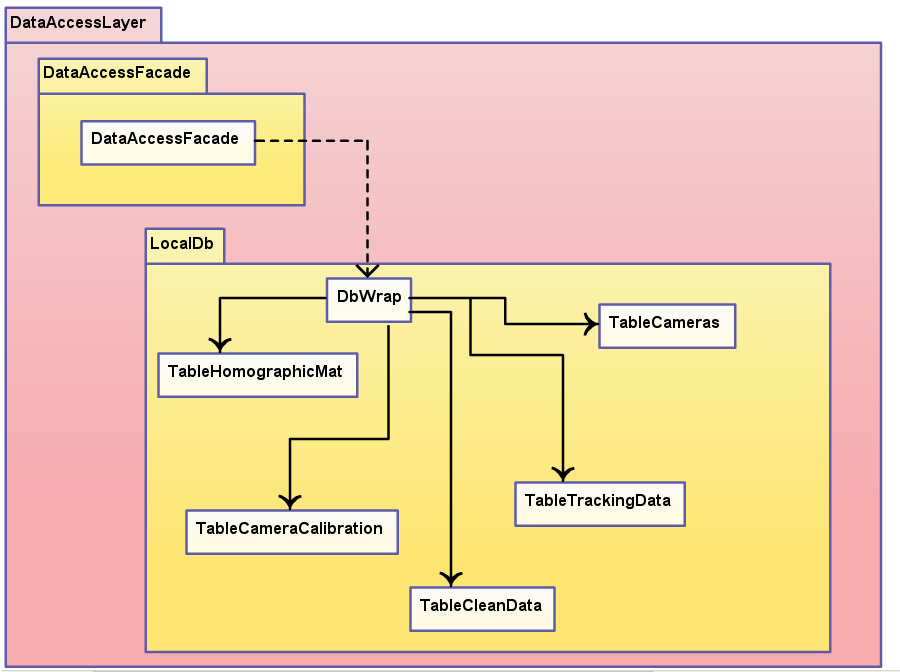
\includegraphics[scale=0.4]{./images/c3.png} 

        \caption{C3 - DataAccessLayer} 

        \label{fig:c3}

        \end{figure} 

\subsubsection{DataAccessLayer::DataAccessFacade} \label{sec:c3.1}
Componente che rappresenta un \textit{facade} per l'effettivo accesso alle funzionalità del \textit{data access layer}. Esso si occupa di fornire una via unificata di accesso per i possibili database differenti con cui l'applicazione si deve interfacciare\\
Relazioni con altri componenti: 
\begin{description} 
\item [\textbf{LocalDb}]
Utilizza LocalDb (~\ref{sec:c3.2}) per accedere ai metodi specifici del database locale, vi inoltra quindi le richieste di insert, update, delete, select 
\end{description} 

Classi contenute nel componente: 
\begin{itemize} 
\item \textbf{DataAccessFacade}
\begin{description}
\item [\textit{descrizione e utilizzo:}] La classe rappresenta un \textit{facade} per l'accesso alle funzionalità del \textit{data layer}. Essa unifica al suo interno tutte le richieste in arrivo dai livelli superiori e le indirizza alla classe appropriata. Viene utilizzata dalle classi del \textit{business layer} per l'accesso ai dati presenti nel database
\end{description}
\end{itemize}

\subsubsection{DataAccessLayer::LocalDb} \label{sec:c3.2}
Componente che contiene le funzionalità per l'accesso al database locale. Esso fornisce l'interfaccia per la modifica dei dati e il loro recupero\\
Classi contenute nel componente: 
\begin{itemize} 
\item \textbf{DbWrap}
\begin{description}
\item [\textit{descrizione e utilizzo:}] Classe wrapper per il database locale contentente le informazioni di configurazione delle telecamere. Essa mette a disposizione i metodi per l'accesso ai dati e la loro modifica. E' implementata come singleton per evitare allocazioni multiple. Contiene una copia statica di tutti i dati presenti nel database, per prevenire accessi ripetuti in memoria che possono causare lentezza del sistema.
\end{description}
\item \textbf{TableHomographicMat}
\begin{description}
\item [\textit{descrizione e utilizzo:}] Classe che contiene i metodi di basso livello per accedere alla tabella \textbf{tbl_homographic_matrices}
\end{description}
\item \textbf{TableTrackingData}
\begin{description}
\item [\textit{descrizione e utilizzo:}] Classe che contiene i metodi di basso livello per accedere alla tabella \textbf{tbl_tracking_data}
\end{description}
\item \textbf{TableCameras}
\begin{description}
\item [\textit{descrizione e utilizzo:}] Classe che contiene i metodi di basso livello per accedere alla tabella \textbf{tbl_cam}
\end{description}
\item \textbf{TableCameraCalibration}
\begin{description}
\item [\textit{descrizione e utilizzo:}] Classe che contiene i metodi di basso livello per accedere alla tabella \textbf{tbl_cam_calibration}
\end{description}
\item \textbf{TableCleanData}
\begin{description}
\item [\textit{descrizione e utilizzo:}] Classe che contiene i metodi di basso livello per accedere alla tabella \textbf{tbl_clean_data}
\end{description}
\end{itemize}

